% THIS IS A LATEX TEMPLATE FILE FOR PAPERS INCLUDED IN THE
% *Anthology of Computers and the Humanities*. ADD THE OPTION
% 'final' WHEN CREATING THE FINAL VERSION OF THE PAPER. 
% DO NOT change the documentclass
\documentclass[final]{anthology-ch} % for the final version
%\documentclass{anthology-ch}         % for the submission

% LOAD LaTeX PACKAGES
\usepackage{booktabs}
\usepackage{graphicx}
% ADD your own packages using \usepackage{}
\sloppy
% TITLE OF THE SUBMISSION
% Change this to the name of your submission


\title{Classification of Script Types and Modes for Medieval Hebrew Manuscripts}

% AUTHOR AND AFFILIATION INFORMATION
% For each author, include a new call to the \author command, with
% the numbers in brackets indicating the associated affiliations 
% (next section) and ORCID-ID for each author.  

\author[1]{Daria {Vasyutinsky-Shapira}}[orcid=0000-0002-4257-7882]

\author[2]{Irina Rabaev}[
  orcid=0000-0002-8542-8342
]

\author[3]{Jihad El-Sana}[
  orcid=0000-0002-1164-7040
]

\author[4]{Ophir Münz-Manor}[
  orcid=0000-0001-6333-345X
]

% While we encourage including ORCID-IDs for all authors, you can
% include authors that do not have one by definining an empty ID.
%\author[2]{Author Three}[
%  orcid=
%]

% There should be one call to \affiliation for each affiliation of
% the authors. Multiple affiliations can be given to each author
% and an affiliation can be given to multiple authors. 
\affiliation{1}{School of Computer Science and AI, Tel Aviv University, Ramat Aviv, Israel}
\affiliation{2}{Department of Software Engineering, Shamoon Academic College of Engineering, Beer-Sheva, Israel}
\affiliation{3}{Department of Computer Science, Ben Gurion University of the Negev, Beer-Sheva, Israel}
\affiliation{4}{Department of History, Philosophy and Judaic Studies, Open University of Israel, Raanana, Israel}

% KEYWORDS
% Provide one or more keywords or key phrases seperated by commas
% using the following command
\keywords{digital paleography, deep-learning models, medieval Hebrew manuscripts}

% METADATA FOR THE PUBLICATION
% This will be filled in when the document is published; the values can
% be kept as their defaults when the file is submitted
\pubyear{2025}
\pubvolume{3}
\pagestart{325}
\pageend{334}
\conferencename{Computational Humanities Research 2025}
\conferenceeditors{Taylor Arnold, Margherita Fantoli, and Ruben Ros}
\doi{10.63744/kHC6jQFdCkNz}  
\paperorder{23}


\addbibresource{bibliography.bib}

%%%%%%%%%%%%%%%%%%%%%%%%%%%%%%%%%%%%%%%%%%%%%%%%%%%%%%%%%%%%%%%%%%%%%%%%%%%
% HERE IS THE START OF THE TEXT
\begin{document}

\maketitle

\begin{abstract}
This paper presents an overview of a few years of work on the automatic classification of types and modes for medieval Hebrew script performed at the VML Lab at the Ben Gurion University. 
We introduce here a new type of paper, a story of how a multidisciplinary team of researchers and students, some leaving in the process and some joining, worked together to solve a challenging problem, interesting as a Computer Science project, and essential for the Humanities research. Our research is pioneering, and it took years of trying and improving. This paper is addressed to a Digital Humanist interested in following the latest advancements in digital Hebrew paleography; it references more technical parts of this work. 
The resulting algorithms and the datasets that were produced in the process are an essential contribution to the automatic layout detection, segmentation, and, eventually, automatic transcription for Hebrew manuscripts. 
\end{abstract}

\section{Introduction} 

Jewish history and culture are deeply woven into European and American cultural heritage, with collections of Hebrew manuscripts in almost all major libraries worldwide. Today, most of these libraries digitize their collections, and thousands of high-resolution manuscript images are already available. Yet, for many users, the digitization has not increased the availability of the manuscripts. To introduce a manuscript into the research, it is not enough to make a digital image publicly available. To make these document images approachable for a broader audience that does not possess the specific paleographical and codicological skills, much pre-processing is required. Before proposing to the end user, a transcription of a text unavoidably includes page layout recognition and segmentation. Effective algorithms exist to deal with simple layouts for printed Hebrew books ~\cite{gogawale2024netlay}. However, for complex layouts, which are a work in progress, detecting the script type-modes would be very helpful, especially when script change is the only change between parts of a text. 

\begin{figure}[t!]
    \centering
    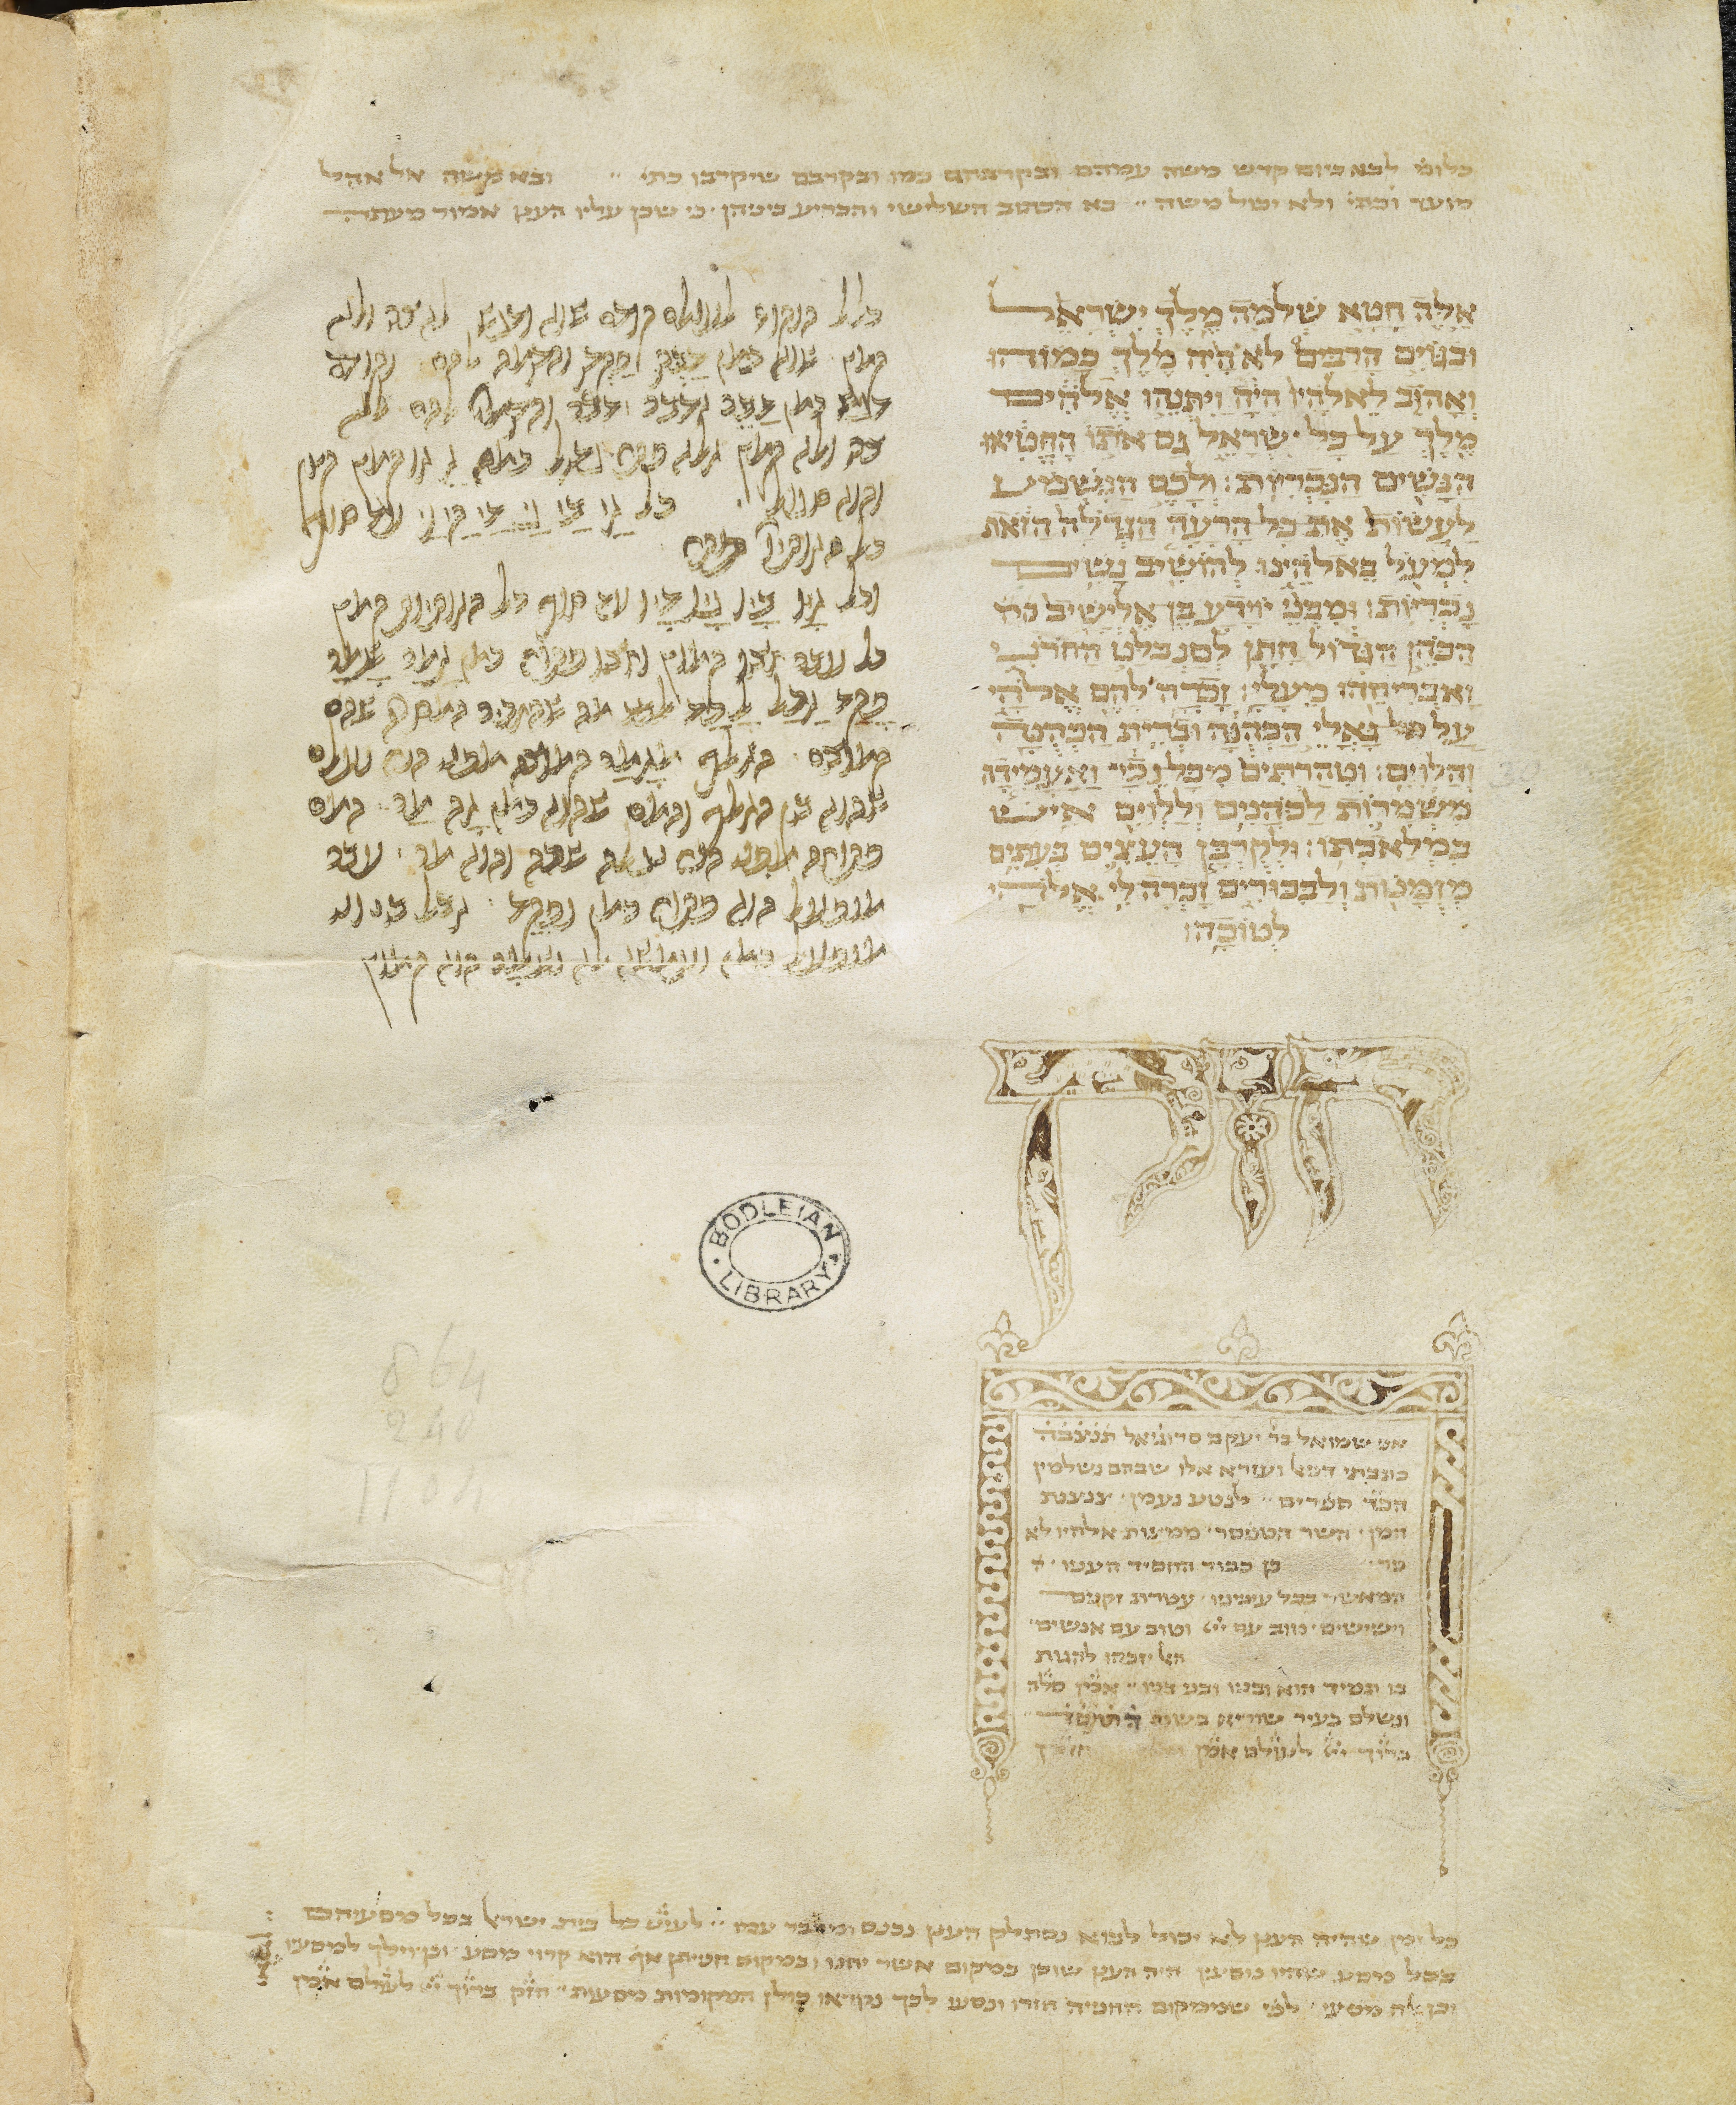
\includegraphics[width=0.40\linewidth]{figures/HebrewBibleSpain1304.jpg}
    \includegraphics[width=0.40\linewidth]{figures/img2.jpg}
    
    \caption{Samples of two Hebrew manuscripts with different script modes on a page. Left: Hebrew Bible, 1304, Sephardic square, semi-cursive, and cursive. Oxford, Bodleian Library MS. Arch. Selden A. 47, fol. 394v: \url{https://digital.bodleian.ox.ac.uk/objects/f1916173-04c4-4fa9-8f4f-ec9eade7f008/}; right: Hebrew Bible, 1335, Ashkenazi square and semi-cursive. Source \url{https://gallica.bnf.fr/}  BnF: \url{https://gallica.bnf.fr/ark:/12148/btv1b10539464v/f119.item}
    }
    \label{fig:MssSamplesl}
\end{figure}

In contrast to printed Hebrew books, that have only two type-modes of script, the Ashkenazi square, and the \textit{Rashi}, in manuscripts we recognize approximately fourteen types of script types and modes: Oriental, Ashkenazi, Italian, Byzantine, and Yemenite regional types with their square, cursive, and the in-between mode (alternatively called semi-square, semi-cursive, and non-square). The founding fathers of Hebrew paleography, such as Malachi Beit-Arié, Colette Sirat, Norman Golb, Benjamin Richler, Edna Engel, and Ada Yardeni  ~\cite{SiratBeitArie1972,EngelBeitArie1987,beit_arie_malachi_2021_8849,sirat2002hebrew,yardeni1997book,richler2011hebrew,richler2008br},  have provided critical insights into the evolution of Hebrew scripts across regions and periods. More current research by Judith Olszowy-Schlanger suggests new paleographic insights~\cite{olszowy2018crossing}. The variability of hands in some type-modes is more pronounced than in others. All these type-modes are extinct today except for Ashkenazi square  (which is today's standard Hebrew print fonts), Ashkenazi semi-cursive (today's standard Hebrew handwriting, with some Italian influence), Sephardic square, and Sephardic semi-cursive (the \textit{Rashi} script). Some of the extinct type-modes are difficult for today's user to read, and some even require special training to decipher. Detecting all these type-modes will definitely help to solve the problem of complex manuscript layouts. Type-mode detection is also essential in automatically recognizing the region of copying, and, as the latest research hints~\cite{atamni2025multi}, can be instrumental in the automatic dating of undated manuscripts. Figure~\ref{fig:MssSamplesl} shows two samples of challenging layouts with multiple medieval Hebrew script type-modes per page.   

Among the ca. 70.000 medieval Hebrew manuscripts, about $5\%$ have a colophon (scriber’s note) that mentions the date and place of copying. We must add ca. 300.000 Cairo Rabbanite Genizah fragments, almost all undated and many of unknown provenance. Most of these manuscripts and fragments remain unstudied. Automatic detection of Medieval Hebrew scripts is an essential first step in introducing these fragments of ancient heritage into the research.   

\section{Related work}
\label{sec:RelatedWork}
Digital paleography exists for several languages, such as Latin, Greek, Hebrew, Persian, English, French, German, Russian, and more. Most of the development of automatic analysis has been geared towards Latin scripts, and many algorithms are intended for left-to-right scripts only. The existing digital Latin manuscripts datasets are by far the biggest, and competitions are regularly held in various types of classification of Latin scripts (ICFHR2016 CLaMM~\cite{cloppet2016icfhr2016}, ICDAR17 CLaMM~\cite{cloppet2017icdar2017}, ICDAR 2021 HDC~\cite{seuret2021icdar}). 

The main concepts for identifying script types in
medieval Latin manuscripts were already proposed in 
2017 in ~\cite{kestemont2017artificial}. The biggest Latin dataset for deep learning was first introduced at the ICFHR2016 Competition on the Classification of Medieval Handwritings in Latin Script (ICFHR16 CLaMM) and enlarged for the ICDAR17 CLaMM.\footnote{\url{https://zenodo.org/record/5527711}} \footnote{The classes of Latin scripts are based on morphological differences, as defined in standard work on Latin scripts~\cite{bischoff1979palaographie}} The training was performed on a set of 3540 images with their ground truths. The CLaMM dataset was used again at the ICDAR2021 Competition on Historical Document Classification (HDC2021) for script recognition~\cite{cloppet2017icdar2017}. Additionally, random pages were taken from 1698 e-codices (9th to 17th cent.) from the Virtual Manuscript Library of Switzerland\footnote{\url{http://e-codices.unifr.ch/}} for the task of dating undated manuscripts, and determining the place of origin was performed on a total of almost 6,000 samples~\cite{seuret2021icdar}. The best-performing algorithm trained on the CLaMM dataset for script type-mode recognition reached almost 89\%  accuracy. The more recent CATMuS dataset, a multitask Latin HTR dataset~\cite{clerice2024catmus}, consists of 200 manuscripts and incunabula. 

The same CLaMM dataset was used for classification of Latin scripts in \cite{boudraa2024revolutionizing,bennour2024heritagescript}. An interested reader can find the overview of the current state-of-the-art for Latin manuscripts in~\cite{lane9modern}.
For Arabic manuscripts, the biggest existing dataset is KERTAS from the Qatar National Library with its 2,502 document images \cite{adam2018kertas}.

\section{Dataset}

Multiple experiments were performed on the same big dataset of Latin manuscripts, because building a new big and balanced dataset (in image quality, quantity, and number of images per type) is one of the most demanding tasks in digital paleography. In Hebrew paleography, the inconsistencies in the raw data are more pronounced because of the low survival rate of the Hebrew manuscripts compared to Latin or Arabic. Hebrew manuscripts were initiated, produced, used, and kept individually and not by formal writing schools (there are, however, indications that there existed commercial workshops for copying manuscripts). The geographical dispersion of Hebrew scripts is more significant than in any other Medieval script, and the state of preservation of Hebrew manuscripts is often worse than that of Latin or Arabic. Moreover, some libraries that hold big collections of Medieval Hebrew manuscripts have not finished the digitization process yet or have not made the digital images publicly available. Among these are libraries of the former Russian Empire, first and foremost the National Library of Russia in St. Petersburg, which keeps the so-called Firkowicz Collections of manuscripts, the oldest and best-preserved Hebrew manuscripts in the world, as well as some of the Italian libraries.  

In digital Hebrew paleography, we often rely on the SfarData\footnote{\url{https://sfardata.nli.org.il/\#/startSearch_En}} dataset of Malachi Beit-Ari\'{e} and his team, which includes all the medieval manuscripts written in Hebrew script. It contains explicit production dates or at least scribe names, with their detailed codicological and paleographical description. Though Malachi allowed our research project full access to the SfarData and its supporting materials, the manuscripts described in the dataset are spread among some 250 libraries worldwide, some private, each with its copyright policy.      

We initially built a small dataset of high-resolution color images, expanding it as we progressed with the research. At the last research stage, we developed the dataset further, using the original b/w images from the Sfardata collection. All the datasets described in this paper are publicly available.

\section{Methodology} 
This section provides a general overview of the methods we used and the results we achieved at different stages of research with each dataset. For in-depth technical details, please refer to the computer science publications listed in the references ~\cite{droby2021vml, droby2022digital,droby2022hard,atamni2025multi}. 

\subsection{Supervised deep learning with the VML-HP dataset} 

\label{sec:supervised_VML-HP}
In 2021, we completed our first dataset, the first ever of this kind built for medieval Hebrew manuscripts. This SfarData-based VML-HP (Visual Media Lab Hebrew Paleography) dataset~\cite{droby2021vml,shapira2022deep} 
consisted of 537 page-images with labels of 15 script type-modes. The page-images were extracted from high-quality digitized manuscripts from the National Library of Israel, the British Library, and the Bibliothèque Nationale de France. For the Oriental square type (presented mainly by the manuscripts of the Firkowicz collections), we used microfilms from the collection of the Institute for Microfilmed Hebrew Manuscripts at the National Library of Israel. The dataset was split into training, typical test, and blind test sets. 

Initially, we started experimenting with supervised deep machine learning, specifically, the Convolutional Neural Network (CNN) models to classify text images into script types  ~\cite{droby2021vml}. 

The input to the model was the patch extracted from the document image, and the output was its corresponding labels (a script type-mode).  The decision to work with image patches instead of individual letters was based on several considerations. First, by analyzing patches, we avoid the need for precise letter segmentation, as automated letter segmentation in medieval manuscripts is challenging and prone to errors. Second, manuscript patches provide a more holistic representation of the document because they capture spatial relationships between adjacent letters, allowing the model to learn patterns that may not be present when focusing solely on individual letters. 

To extract patches that contain enough information, we developed a dedicated patch generation tool that generates image patches with approximately five text lines, avoiding patches with severe image noise, paintings, and patches with no or little text ~\cite{droby2021vml}
. 
Irrelevant background features could hinder the training process. Therefore, before feeding the patches into the network, they underwent pre-processing by applying bilateral and low-pass filters. The filtering reduced the background information passed to the network. 

We experimented with different network architectures
for classifying script type-modes: DenseNet, 
AlexNet, VGG11, ResNet50, and SqueezeNet. The 
ResNet50 classifier showed the best performance with $42.1\%$ and $49.3\%$ accuracy at the patch and page levels, respectively.  The final page prediction was defined as the majority vote of the patches sampled from this page. The results of these experiments were not satisfactory, and after performing an in-depth analysis, we concluded that they hinted at inconsistencies in the dataset on the paleographical side (especially Yemenite semi-cursive type-mode, one of the type-modes understudied in classical paleography, and underrepresented in the SfarData, caused numerous errors).  

\subsection{Soft labeling}

After consulting with Malachi Beit-Ari\'{e}, the Yemenite semi-cursive type-mode was dropped, some manuscripts were replaced, and the dataset was enlarged. The resulting VML-HP-ext (Visual Media Lab Hebrew Paleography Extended) dataset contained $715$ page-images excerpted from $171$ manuscripts equally representing fourteen script type-modes  ~\cite{droby2022digital,droby2022hard}. 

Some of the limitations of the raw data were derived from our inability to use the codicological data. In the SfarData, script type and mode were manually defined based on combined codicological and paleographical data , while our models use paleographical data only. We tried to introduce an alternative level of labeling -- a soft label -- for each page. The soft level is represented by a label vector, where each element specifies the degree of similarity between the processed document and the specific script type or mode. In our experiments, we utilized a vector of size eight, each element of which is in the range [0,1].
The first six elements of the vector express the degree of similarity of the manuscript to a certain regional type, and the last two elements are the degrees of similarity to either square or cursive graphical mode (similar values for both square and cursive indicate the semi-cursive mode). The soft-labeling was performed by the team's Hebrew paleographer.

 For these experiments, we used a regression model with a ResNet50 backbone ~\cite{droby2022hard}. 
The predicted soft levels were converted to hard labels to evaluate and compare the results. The soft-label regression model obtained an accuracy of $67\%$ using the regional style labels, but overall did not reach the accuracy of the models trained using hard-labeling. 

\subsection{Supervised deep learning on the extended dataset}

Similar to the experiments presented in Section~\ref{sec:supervised_VML-HP}, we adopted a CNN model to classify patches extracted from the pages in the VML-HP-ext dataset. The models consisted of two components: an established CNN backbone (e.g., ResNet, VGG), which acted as a feature extractor, followed by two fully connected layers. In addition, to find the best input format, we experimented with several types of input: grayscale, binary, and smoothed patches. The model trained with binary patches achieved the highest accuracy of $62\%$. 

After determining the best input format, we experimented with different CNN backbone architectures: VGG19, DenseNet, several ResNet versions, and AlexNet. The models were trained and tested using binarized patches. Upon completion of the experiments, VGG19 showed the best performance, reaching an accuracy of $66\%$ on the patch-level classification, $70.4\%$ on the page level.  DenseNet and ResNet versions reached similar accuracy, about $62\%$. AlexNet did not perform as well as the rest, reaching an accuracy of $53\%$. We explain these results by considering the complexity of each model. A simple model may not have the capacity to learn the classification problem, but is less likely to overfit on the training set. In contrast, a more complex model can learn more complex problems but is more likely to overfit. We concluded that VGG19 is complex enough to reach $66\%$ accuracy and simple enough to avoid overfitting. 

Looking deeper into the results, we saw that the model did not make "rough" mistakes, it did not misclassify type-modes that are very different. It rather struggled to classify Italian square and semi-cursive, confusing them with Ashkenazi and Byzantine square and semi-cursive. These errors also arise in manual labeling, as these type-modes can be confused by a human paleographer, too.  

To solve the confusion mentioned above, we experimented with separately classifying the regional styles and graphical modes. We trained two VGG19 models to classify the regional styles and graphical modes. Both models were trained using the same training scheme as the previous experiments. The model trained to classify the regional styles reached an accuracy of $81\%$ at the patch level and $85\%$ at the page level. The model trained to classify the graphical modes reached an accuracy of $77\%$ at the patch level and $80\%$ at the page level. This result, though satisfactory, required further research with new approaches.  

To further evaluate the model's effectiveness, we compared its accuracy with an expert's. For this, we compiled an online questionnaire. We asked an experienced paleographer who was not part of our team and was not deeply involved in building the SfarData to classify 75 manuscripts' patches. The patches were randomly chosen from the set used in our experiments, approximately five from each class. The accuracy rate of the paleographer was $70\%$. It should be noted that the problem was challenging for the human expert due to the unusual format: paleographers work with manuscripts and pages, not patches. 

\subsection{Unsupervised deep learning}

Next, we attempted to take another step toward fully automatic solutions. We utilized unsupervised learning to train the model without explicit class labels. In the experiments described in previous sections, each training sample was represented by a document patch and its corresponding script type-mode label. For the unsupervised approach, the input to the model was given by a pair of document patches and a binary label. The binary label indicates if the pairs are from the same or different classes. The experiments were conducted on the VML-HP-ext 
dataset using the same patch extraction algorithm as before. The input included positive and negative pairs of patches, i.e., pairs of patches corresponding to the same class and pairs of patches from different classes. Since the training did not utilize explicit classes (script-type modes), we classified this approach as unsupervised learning.

For the experiments, the Siamese network was utilized to learn the similarity of pairs of input images. The features of the trained Siamese network were then passed to a clustering algorithm to construct the desired number of clusters (the number of classes we wanted to get at the end of the experiment).

We studied the performance of our method with various cluster sizes, and increasing the number of clusters improved the accuracy of our model. Compared with a supervised approach that classified our dataset into 14 classes, the unsupervised model showed an accuracy of 0.65 on the patch level. This is a satisfactory result, but it did not reach the level of accuracy of the supervised model.   

\section {Script classification and dating}

We recently took a new approach to the dataset and the research problem. We enlarged the dataset radically and addressed the style classification and the dating problems together ~\cite{atamni2025multi}. 

Instead of manually building a dataset of high-resolution color images available in different libraries, we extracted from the SfarData the original images, b/w photos from the 1970s-1990s. These images always include the colophon page, frequently written in a different script mode than the main text. When preparing the dataset, the team's paleographer picked up the pages with only one script type-mode per page, and only these pages were used in our experiments. 

This resulted in the VML-MHS (Visual Media Lab - Medieval Hebrew Sfardata) 
dataset, which includes fragments from 2,304 manuscripts, 3,687 page-images total. Each manuscript in the dataset was labeled with its script type, mode, and precise year of copying, offering rich metadata for comprehensive paleographic analysis. Manuscripts were now categorized with labels in the format "Script style/Script Mode/Date" (e.g., Oriental/Square/1040), embedding the temporal aspect directly into the dataset structure.
Spanning 1266 unique years from 850 CE to 1540 CE, the dataset was divided into folders, each folder representing a specific year. 

Similar to the previous experiments, we extracted from the page-images over 346,000 document patches for detailed script analysis. 

This recent work proposes a multi-task transformer-based framework that jointly addresses Hebrew script classification and manuscript dating, which is a clear departure from our team's earlier work, which relied on CNN-based models (e.g., ResNet, EfficientNet) where we classified the script type-mode separately. We proposed a multi-task learning (MTL) approach that performs script classification and manuscript dating jointly. Instead of treating these tasks independently, our model builds robust generalization capabilities by learning shared feature representations from diverse domains, encompassing different script types and temporal (date) domains. The model’s architecture consists of three main components: 
\begin{enumerate}
   \item A Transformer-Based Backbone: The backbone serves as a high-level feature extractor, leveraging vision transformer architectures (e.g., ViT, Swin, BEiT). These models are pre-trained on large-scale datasets and then fine-tuned on our dataset. The input image patches are tokenized and then processed through multiple self-attention layers, capturing local and global contextual relationships within handwriting patterns. The extracted feature representations are then shared across both the classification and regression heads, ensuring optimal learning across different tasks.
    \item A Script Classification Head: This branch is responsible for identifying both the script's type (e.g., Ashkenazi, Byzantine, Italian) and its mode (Square, Semi-Cursive, Cursive).
    \item A Date Estimation Head: This branch estimates the production time of a manuscript by classifying it into historical periods, regressing it to decade intervals based on the year.
\end{enumerate}

We grouped manuscripts into decades for date estimation because the manuscripts are not evenly represented throughout the years. By estimating the decade instead of years, we encouraged the model to generalize better and smoothly interpolate the missing dates. The best-performing model (Swin-Base) achieved $90.5\%$ classification accuracy for script type and a mean decade error of 4.88 (the average deviation between the predicted and actual decade for manuscript date estimation). In the script classification, the algorithm performed very well on most scripts, with lower performance for Byzantine Square (71.4\%) and Sephardic  Square (60\%), indicating complex challenges in these categories that we'll still have to address in the future. 

Our latest results demonstrate substantial gains in both accuracy and temporal depth over earlier CNN-based methods and suggest that it might be advantageous to classify both script and date simultaneously. Each of the medieval Hebrew scripts developed at its own pace. They were influenced by other Hebrew scripts and the local scripts, too, but forms of letters evolved for each script differently. Thus, classifying the date and the script together might lead to better results for both.  

\section{Conclusions and Future Work}

In this paper, we presented the research done by our team for the automatic detection of Medieval Hebrew scripts as part of our effort to provide automatic solutions for the analysis of digitized historical documents. We have conducted numerous experiments with supervised and unsupervised learning, with hard and soft labels. We have reached excellent results in both automatic script detection and automatic dating. 

We have concluded that deep-learning models can efficiently produce fully automatic research tools for the analysis and research of medieval manuscripts. 

Further advancements in the field can be reached by introducing a large-scale dataset of high-resolution color images based on the Ktiv project of the National Library of Israel. This task, very costly in work-hours and involving multiple copyright issues, remains a big \textit{desideratum} in the digital Hebrew paleography.



\section*{Acknowledgements}

The research was performed at the Visual Media lab of Ben-Gurion University of the Negev. The authors are grateful to Dr. Ahmad Droby, Dr. Berat Kurar Barakat, and Reem Alasam for their significant contribution to this study as part of their research at the VML lab.

The participation of Dr. Daria Vasyutinsky Shapira was supported by Yuval Ne'eman scholarship for postdoc research in Digital Humanities of the Israeli Ministry of Science and Technology (grant n. 3-16784, 2020-2022); Postdoctoral grant of the Center for Digital Humanities at the Open University of Israel (2022-2023); European Union (ERC, MiDRASH, Project No.\@ 101071829, since 2023). Views and opinions expressed are, however, those of the author only and do not necessarily reflect those of the European Union or the European Research Council Executive Agency. Neither the European Union nor the granting authority can be held responsible for them.  

% Print the biblography at the end. Keep this line after the main text of your paper, and before an appendix. 
\printbibliography

\end{document}
